
\section{Politique de distribution de l’espace d’états basée sur le	comportement du système}
 
La politique proposée, vise à optimiser la distribution de l’espace d’états ainsi que le temps de vérification du model checking. Pour un système donné spécifiée à partir d'un réseau de Petri, nous utilisons un algorithme de génération parallèle pour construire la structure de Kripke distribuée, en utilisant la fonction \emph{MD5} pour le partitionnement de l’espace d’états entre les machines du réseau. Après cela, lors de l'exécution du model checking, chaque machine analyse son fragment (structure de Kripke partielle) et élabore certaines statistiques sur les états par rapport à la vérification. Les statistiques  générés sur chaque état mesure la dépendance de l'état par rapport aux états de la machine locale ou aux états des machines distantes. Une fois le processus de vérification du model checking est terminé, le protocole de redistribution peut être lancé afin de calculer l'ensembles des états à déplacer et à dupliquer pour chaque état \emph{Externe} et \emph{sollicité}. Après le calcul des ensembles on décide, sur la base de l'écart minimum et maximum des états à stocker sur la machine, si l'ensemble peut être déplacé ou resté dans une machine afin de minimiser la taux de communications entre les machines tout en garantissant une bonne distribution. Ainsi, une bonne distribution n'implique pas la réduction des transitions reliant les parties.


L’algorithme général est l'Algorithme \ref{bbssd} :\\
\begin{algorithm}[H]\label{bbssd}
	\SetAlgoLined
	\SetKwIF{If}{ElseIf}{Else}{if}{then}{else if}{else}{endif}
	 Générer la structure de Kripke distribuée à partir de la spécification d'un réseau de Petri\;
	 Exécution du model checking et élaboration des statistiques sur chaque état\;
	 Redistribuer les états en optimisant les performances du système\;	  
	\caption{\CDS{}}
\end{algorithm}
Dans les sections suivantes, nous détaillons les phases de cet algorithme.

 
\begin{figure}[h]
	\centering
	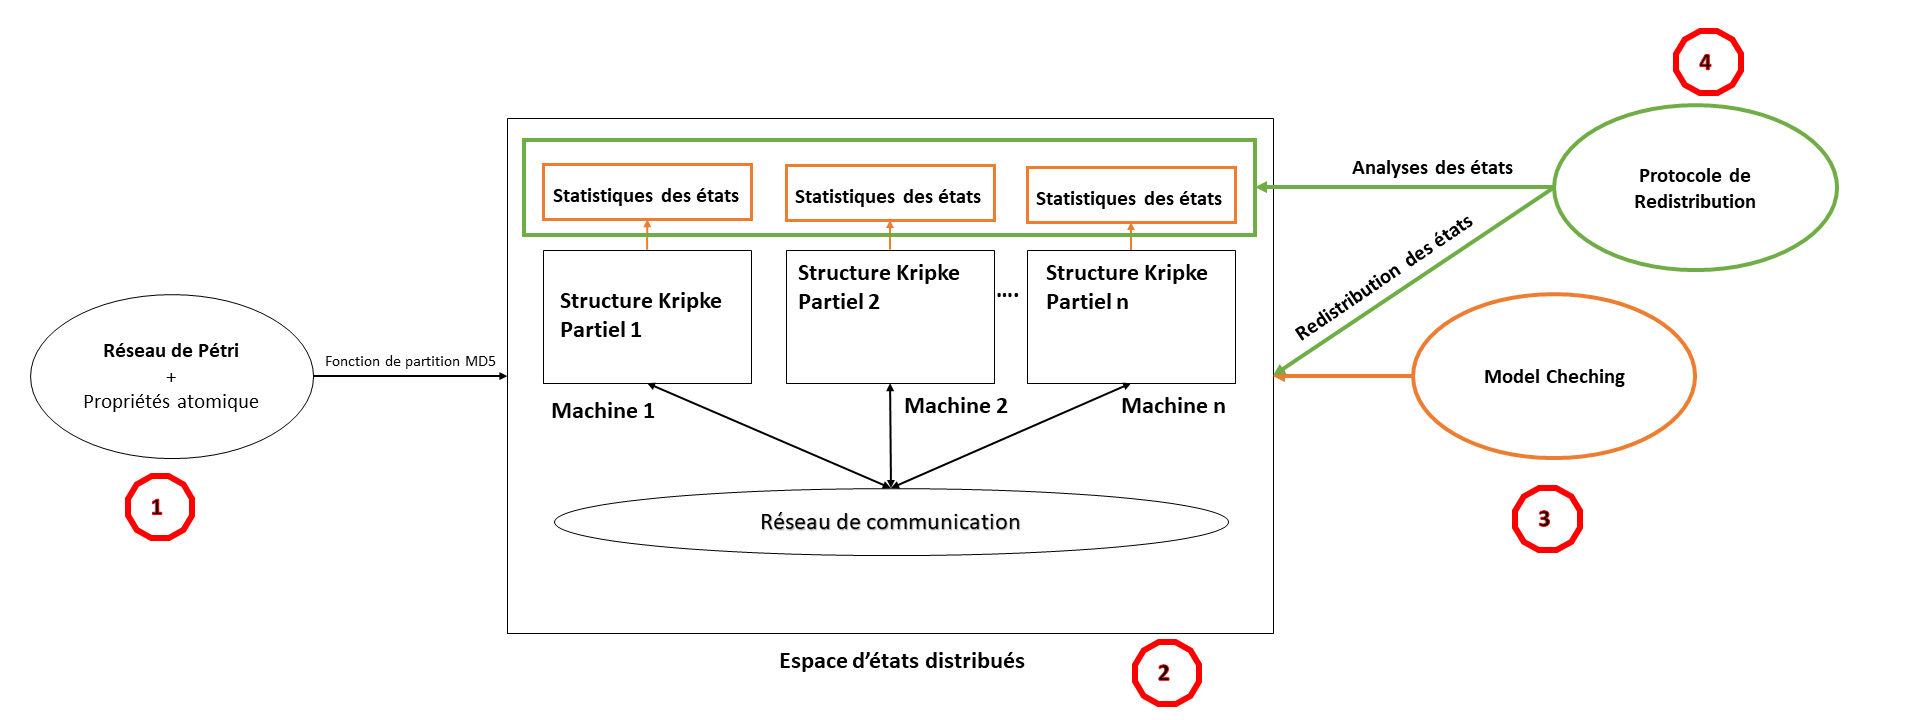
\includegraphics[height=3.0in,width=1.0\textwidth]{img/protocole}
	\caption{Schéma de la politique de redistribution de l'espace d’états}
\end{figure}
	
 

\subsection{Génération distribuée de l’espace d’états à partir de la spécification d'un réseau de Petri}{
La spécification du réseau de Petri est faite à partir d'une machine choisie aléatoirement. Le processus de génération distribuée de l'espace d'états est fait par l’exploration de l’état initial en générant tous ses états successeurs. Par la suite, toutes les machines disponibles sur le réseau contribuent à la construction des fragments de l’espace d’états distribué. Pour chaque nouvel état généré appartenant à une machine $M_i$, tous ses états successeurs sont générés. Un état successeur peut être dans la même machine ou dans une machine distante. Chaque machine $M_i$ envoie tous ses états externes aux machines déterminées par la fonction de partition. La fonction de partition est basée sur la fonction de hachage cryptographique \emph{MD5} qui renvoie un index $j\;(j \in 0, N-1)$. La fonction de hachage adoptée réalise un bon équilibrage de charge entre les $N$ machines du réseau.  La génération distribuée se termine lorsqu'il n'y a aucun états en attente d'être exploré.\\
L’algorithme de génération distribuée de l’espace d’états est l'Algorithme \ref{gendistribuer} :\\
\SetKwFunction{printlcs}{}
\begin{algorithm}
	\SetAlgoLined
	\SetKwIF{If}{ElseIf}{Else}{if}{then}{else if}{else}{endif}
	\SetAlgoLined	
	\SetKwInOut{Mi}{$M_i$}
	\SetKwInOut{Mj}{$M_j$}
	\SetKwInOut{etati}{$Etat_i$}
	\SetKwInOut{ei}{$E_i$}
	\SetKwInOut{si}{$S_i$}
	\SetKwInOut{t}{$t$}
	\SetKwInOut{T}{$T$}
	\SetKwInOut{smm}{$s,m,m'$}
	\SetKwInOut{tb}{$t_b$}
	\SetKwInOut{sm}{$s.m$}
	\SetKwInOut{sprp}{$s.L$}
	\SetKwInOut{te}{$TExplore$}
	\SetKwInOut{tr}{$TR_i$}
	\SetKwInOut{Pres}{$Pres$} 
	\SetKwInOut{Post}{$Post$}
	\SetKwInOut{pps}{$Prop\_Pres$}
	\SetKwInOut{ppt}{$Prop\_Post$}
	\AlgoDontDisplayBlockMarkers\SetAlgoNoEnd\SetAlgoNoLine%
	\Mi{machine i}
	\Mj{machine j}
	\etati{\{dehors,dedans\}}
	\ei{init à $\emptyset$, pile des états non encore explorés appartenant à la machine i}
	\si{init à $\emptyset$, la liste des états déjà explorés appartenant à la machine i }
	\smm{un état}
	\sm{marquage d'un états}
	\sprp{liste des propriétés d'un états}
	\tr{la liste des relations de transitions de la machine i}
	\T{a liste de transitions}
	\tb{transition bloquant}
	\te{liste transition admissible}
	\t{une transition}
	\Pres{matrice pres du réseau de Petri}
	\Post{matrice post du réseau de Petri}
	\pps{matrice pres des propriétés}
	\ppt{matrice post des propriétés}

	 \caption{Génération Initiale Distribuée}\label{gendistribuer}
 
	\SetKwFunction{algo}{}\SetKwFunction{proc}{proc}
	\Begin{	 
	 \SetKwProg{myalg}{Reception Etat}{}{}
	 
	 \myalg{\algo{m:etat}envoyé par $M_j$}{  
	 	$s\leftarrow findByMarquage(m,S_i)$\;	
	 	\uIf{($ s ==null$)}{
	 		$m.sub\leftarrow\{ M_j \}$\;
	 		Empiler(m,$E_i$)\;	 		
	 		\If{($Etat_i$!= dedans)}{
	 			GenerationDistribue$_i$()\;
 			}
	 	}
 		\Else{
 		   ajouter $M_i$ à la liste des machines de l'etat portant identifiant \emph{m} \;			
 		}	 		  		
	 }{} 	  	
   	\SetKwProg{myalgone}{GenerationDistribue$_i$}{}{}   
  	 \myalgone{\algo{}}{  
	  	$Etat_i\leftarrow dedans$\;	
	  	\While{($ E_i !=\emptyset$)}{
	  		$m\leftarrow depiler(E_i)$\;
	  		$TExplore \leftarrow \{t\in T\mid m.m[t>\}$\;
	  		$S_i\leftarrow S_i \cup \{m\}$\;
	  		\ForEach{($t \in TExplore$)}{
	  			$m'.m\leftarrow m.m + Post(t)-Pres(t)$\; 
	  			$m'.L\leftarrow m.L + Prop\_Post(t)-Prop\_Pres(t)$\; 
	  			$M_j \leftarrow MD5(m'.m)$\;
	  			\uIf{$M_j = =M_i$}{
	  				$s\leftarrow findByMarquage(m,S_i)$\;
	  				\If{(findByMarquage(m'.m,$S_i$)==null and findByMarquage(m'.m,$E_i$)==null)}{
	  					Empiler(m',$E_i$)\;
	  				}
  				}\Else{  				
  					Envoyer (m') à $M_j$\;
  				}
  				$TR_i\leftarrow TR_i\cup \{(m,t,m')\}$	\;
  			}	
	  			
	  		\If{(TExplore== $\emptyset$)  }{
	  		 	$TR_i\leftarrow TR_i\cup \{(m,t_b,m)\}$\;
	  		}
  		}
	  	$Etat_i\leftarrow dehors$\;
	  }{}
  }
\end{algorithm}
\begin{algorithm}
	\LinesNumbered
	% This is to restore vline mode if you did not take the package as \usepackage[linesnumbered,ruled,vlined]{algorithm2e}
	\SetAlgoVlined 
 	 \SetKwProg{myalgone}{Initialisation}{}{ }
  	 \myalgone{\algo{}}{  
  	 $T\leftarrow init$\;
  	 $Pres\leftarrow init$\;
  	 $Post\leftarrow init$\;
  	 $Prop\_Pres\leftarrow init$\;
  	 $Prop\_Post\leftarrow init$\;
  	 $m.m\leftarrow init$\;
  	 $m.prop\leftarrow init$\;
  	 $M_i \leftarrow MD5(m.m)$\;
  	 Envoyer (m) à $M_j$\;
  
  }
	
\end{algorithm} 
}
\pagebreak
%%%%%%%%%%%%%%%%%%%%%%%%%%%%%%%%%%%%%%%%%%%%%%%%%%%%%%%%%%%%%%%%%%%%%%%%%%%%%%%%%%%%%%%%%%%%%
%%									section 1.	Principe Mod\`{e}le Checker Distribu\'{e}											%
%%%%%%%%%%%%%%%%%%%%%%%%%%%%%%%%%%%%%%%%%%%%%%%%%%%%%%%%%%%%%%%%%%%%%%%%%%%%%%%%%%%%%%%%%%%%%

\subsection{Principe du Model Checking Distribu\'{e}}
 
Le model checking adopté est celui qui a été  propos\'{e} par Bouneb Zine dans sa thèse \citep{depriester2011bouneb} (voir chapitre \ref{chapmc}, section \ref{mcd}), permet une vérification parallèle d’une formule $\varphi$  sur les fragments de la structure de Kripke distribuée. Du fait de la distribution, la vérification de $\varphi$ d'un certain état \emph{S} dépend de la vérité en \emph{S’} de cette formule, \emph{S’}  hébergé dans une  machine distante $M_j$. La machine $M_i$ effectue la vérification de $\varphi$ sur le fragment détenue en considérant la valeur logique de \emph{S’} indécidable  $L (\emph{S’},\varphi )=\perp$ car la formule $\varphi$ peut être vérifiée en \emph{S’}. Lorsque la machine $M_j$ termine le calcul est que la formule est vérifiée en \emph{S’}, aucune notification n'est envoyée à la machine $M_i$, la machine $M_i$ considère que la formule est vérifiée en \emph{S’}, sinon la machine $M_j$ envoi à la machine $M_i$ la valeur logique de \emph{S’} qui est $L(\emph{S’}, \varphi) =false$. Dans ce cas, $M_i$ reprend le calcul de vérification avec la prise en compte de valeur logique envoyée afin de déterminer la logique de formule sur les états prédécesseurs. Une fois la terminaison est détectée, la machine détenant l’état initial déduit la véracitée de la formule $\varphi$.

\begin{Exemple}
   Soit une structure de Kripke distribuée représentée sur la Figure \ref{skd1}, les scénarios de l'exécution du model checking de la formule \s{AG(a)} sur cette structure sont:
   \begin{itemize}
   	\item Après une première itération l'algorithme détecte sur la machine $M_1$ que la formule n’est pas vérifiée sur l’état \s{S1}, cela nécessite l'envoyer d'une notification à la machine $M_3$ qui possède un prédécesseur direct de cet état.
   	\item Après la réception d'une notification sur la machine $M_3$ et la prise en compte de la notification sur l'état \s{S1}, l'algorithme du model checking est relancé sur la machine $M_3$. Après le processus de vérification, la valeur logique de la formule sur l’état \s{S5} est $false$ grâce à la deuxième itération. Après cela, aucune notification n'a été envoyé, sur la machine $M_3$ l'algorithme déduit alors la véracitée de la formule.
   \end{itemize}    
Les résultats observés durant le processus de vérification de la formule \s{AG(a)} sont représentés dans le Tableau \ref{statistique}, les lignes représentent les données concernant un état et les colonnes les types de données construits durant le processus de vérification. Les abréviations utilisées sont:
\begin{description}[,leftmargin=2cm,labelindent=1em]
	\item[Id   :] L'identifiant de l’état;
	\item[VL   :] La valeur logique de la formule à vérifier $(true : 1 ; false : 0 ; \perp : -1)$;
	\item [Sub :] Liste des machines sollicitant l'état;
	\item[T    :] Le type d’état (I : interne ; E : externe);
	\item[Site :] La machine distante o\`{u} l'état (Externe) réside;
	\item[I    :] La liste des itérations permettant de déterminer la valeur logique de l'état.	
\end{description}
   \centering
	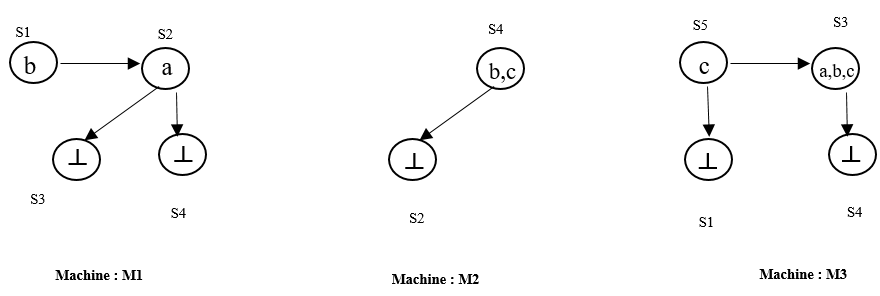
\includegraphics[height=2in]{img/skd1.png}	
	\captionof{figure}{Structure de kripke distribu\'{e}}\label{skd1}
\end{Exemple}
\begin{tableth}
	\centering
	\begin{tabular}{|c|c|c|c|c|c|c|c|c|}
		\hline
		\multicolumn{7}{|c|}{Itération 1}                                  \\ \hline
		          Machine           & Id & T & VL & I & Site &    Sub      \\ \hline
		\multirow{4}{*}{Machine M1} & S1 & I & 0  & 1 &      & \{$M_3$\}   \\ \cline{2-7}
		                            & S2 & I & -1 & 1 &      &             \\ \cline{2-7}
		                            & S3 & E & -1 & 1 &  M3  &             \\ \cline{2-7}
		                            & S4 & E & -1 & 1 &  M4  &             \\ \hline
		\multirow{2}{*}{Machine M2} & S2 & E & -1 & 1 &  M1  &             \\ \cline{2-7}
		                            & S4 & I & -1 & 1 &      &             \\ \hline
		\multirow{4}{*}{Machine M3} & S4 & E & -1 & 1 &  M2  &             \\ \cline{2-7}
		                            & S5 & I & -1 & 1 &      &             \\ \cline{2-7}
		                            & S3 & I & -1 & 1 &      &             \\ \cline{2-7}
		                            & S1 & E & -1 & 1 &  M1  &             \\ \hline
		\multicolumn{7}{|c|}{Itération 2}                                  \\ \hline
		\multirow{2}{*}{Machine M3} & S1 & E & 0  & 2 &  M1  &             \\ \cline{2-7}
		                            & S5 & I & 0  & 2 &      &             \\ \hline
	\end{tabular}
	\caption{Statistique des \'{e}tats}\label{statistique}
\end{tableth}


%%%%%%%%%%%%%%%%%%%%%%%%%%%%%%%%%%%%%%%%%%%%%%%%%%%%%%%%%%%%%%%%%%%%%%%%%%%%%%%%%%%%%%%%%%%%%
%%									section .	2.	Param\`{e}tre d’optimisation									%
%%%%%%%%%%%%%%%%%%%%%%%%%%%%%%%%%%%%%%%%%%%%%%%%%%%%%%%%%%%%%%%%%%%%%%%%%%%%%%%%%%%%%%%%%%%%%

\subsection{Paramètres d’optimisation}
 
Après une analyse du principe précèdent nous avons constaté que la distribution des états liés entrainent un nombre de calculs assez élevé pour déterminer la valeur logique de la formule sur ces états. Le regroupement de ces états améliore le temps de traitement, cela nécessite la prise en considération des objectifs fixés pour éviter la centralisation. Ainsi, les paramètres $\parametreone{}$, $\parametretwo{}$ et $\parametretree{}$ sont utilisés pour atteindre ces objectifs. La prise en compte simultanée des trois paramètres permet de minimiser à la fois le temps de traitement et assurer l’équilibrage de charge avec un nombre réduit de dupliquâts. La résolution de ce problème entraine l'utilisation de fonctions objectives qui permet de trouver l'espace de solutions admissibles car il peut existé une infinité de configurations respectant ces contraintes. Ainsi, différentes techniques sont offertes pour l'obtention de l'espace des solutions, dans ce contexte la technique d’équilibre de Nash combinée aux fonctions objectif est envisageable.
\begin{description}[leftmargin=*,labelindent=1em]
	\item[$\parametreone{}$] Le paramètre de temps de traitement;
	\item [$\parametretwo{}$] Le paramètre d'équilibrage de charge entre les machines ;
	\item [$\parametretree{}$] Le paramètre de dupliquâts  entre les machines.
\end{description}



%%%%%%%%%%%%%%%%%%%%%%%%%%%%%%%%%%%%%%%%%%%%%%%%%%%%%%%%%%%%%%%%%%%%%%%%%%%%%%%%%%%%%%%%%%%%%
%%									section :	Principe d’\'{e}quilibre de Nash					%
%%%%%%%%%%%%%%%%%%%%%%%%%%%%%%%%%%%%%%%%%%%%%%%%%%%%%%%%%%%%%%%%%%%%%%%%%%%%%%%%%%%%%%%%%%%%%

 \subsection{Principe de l’\'{e}quilibre de Nash}
 
L'\'{e}quilibre de Nash est une solution propos\'{e}e par John Forbes Nash en 1950 \citep{depriester1950johnnash} pour la recherche d’une solution optimale. Il est couramment utilis\'{e} en th\'{e}orie des jeux. Un jeu pr\'{e}sente une combinaison de d\'{e}cisions individuelles, appel\'{e}es «strat\'{e}gies», où chaque joueur anticipe correctement les choix des autres; Il y a autor\'{e}alisation, puisque l'issue r\'{e}alis\'{e}e est le fruit de d\'{e}cisions prises en pensant qu'elle va se r\'{e}aliser. En th\'{e}orie des jeux la question que se pose un joueur au moment de faire son choix est : que va faire l'autre ? Ses croyances concernant le comportement des autres joueurs ont donc un rôle essentiel au moment de la d\'{e}cision. La diversit\'{e} de croyance correspond ainsi \`{a} une multiplicit\'{e} d'\'{e}quilibres. Dans les jeux coop\'{e}ratifs on autorise la communication et les accords entre joueurs avant la partie, les messages formul\'{e}s par un joueur sont transmis sans modification \`{a} l'autre joueur, les accords entre joueurs seront respect\'{e}s, ces hypoth\`{e}ses permettent d'obtenir un \'{e}quilibre de Nash.

En utilisant le principe de Nash, J.A D\'{e}sid\'{e}ri \citep{depriester2007jeanantoine} propose un algorithme de partitionnement de territoire qui se base sur des fonctions objectifs. Il consid\`{e}re le cas où on dispose des fonctionnel pr\'{e}pond\'{e}rantes, ainsi l'algorithme cherche \`{a} optimiser les fonctions prioritaires avec une moindre d\'{e}gradation tout en associant aux fonctionnelles secondaires des param\`{e}tres qui engendrent de grandes variations. La recherche de l’\'{e}quilibre de Nash se fait par \'{e}change de r\'{e}sultats obtenus pour chaque fonction objectif travaillant avec une partie seulement des variables, les autres \'{e}tant fix\'{e}es par les r\'{e}sultats obtenus pour les autres fonctions objectifs. Cet \'{e}quilibre est atteint quand l’optimisation de chaque fonction conduit toujours \`{a} la m\^{e}me solution.

En s'inspirant de ces principes, on propose une strat\'{e}gie d'optimisation des param\`{e}tres définie ci-dessus.
%%%%%%%%%%%%%%%%%%%%%%%%%%%%%%%%%%%%%%%%%%%%%%%%%%%%%%%%%%%%%%%%%%%%%%%%%%%%%%%%%%%%%%%%%%%%%
%%									section 4.	Principe de Optimisation (α, \beta, \gamma)								%
%%%%%%%%%%%%%%%%%%%%%%%%%%%%%%%%%%%%%%%%%%%%%%%%%%%%%%%%%%%%%%%%%%%%%%%%%%%%%%%%%%%%%%%%%%%%%

\subsection{Principe d'Optimisation de $\alpha, \beta\; et\; \gamma$}
 
Dans le cadre du model checking, les états présentent des informations par rapport à la vérification. L’analyse de ces résultats, montre que la distribution des états fortement liés augmente le temps de traitement de la vérification. A titre d'exemple sur l'exemple précédente, la distribution des états $S1$ et $S5$ a augmenté le temps de la vérification du model checking car ces états sont liés. Dans un exemple plus complexe o\`{u} un ensemble d’états liés sont distribués, le temps de la vérification sera très élevé. Pour avoir une distribution de l'espace d'états respectant les objectifs fixés nous optimisons les paramètres $\alpha, \beta \; et\; \gamma$ en simulant un jeu non coopératif entre les machines. L'optimisation de ces paramètres est faite comme suit:
\begin{itemize}
	\item Sur Chaque machine on recherche le nombre d'états liés à chaque état sur lequel la formule n'est pa vérifiée, le paramètre $\beta$ pour cet état est égale à ce nombre. Les états local qui disposent des prédécesseurs directs sur d'autres machines distantes, la valeurs du paramètre correspond aux nombres des successeurs directs et indirects liés au même états.
	\item La limite des états liés ou dépendant peut entraîner la duplication de certain états, ce nombre états correspond à la valeur du paramètre $\gamma$. 
	\item En appliquant une heuristique sur les paramètres $\beta \; et\; \gamma$ de deux machines qui sont liées par un état nous obtenons une optimisation du paramètre $\alpha$.
\end{itemize}
Dans les sections suivantes, nous détaillons les phases de ce principe d'optimisation, la structure de Kripke présentée sur la Figure \ref{skd2} sera utilisée dans les exemples. \\

A partir du nombre d'états stockés dans chaque machine il est possible de calculer le nombre minimum et maximum d’états susceptibles d’être stockés par deux machine. Le calcul de cet interval est comme suit :

\begin{itemize}
	\item  	Soit $(\beta1 \; et\; \gamma1)$ les valeurs de la machine $M_1$ respectivement pour la machine $M_2$ $(\beta2 \;et\; \gamma2)$.
	\item  	$\overline{\beta}$ la moyenne des états $\overline{\beta}=\frac{\beta1+\beta2}{2}$.
	\item  	L’écart type $\delta=\sqrt{\frac{\displaystyle\sum_{i=1}^{2}\beta_i^2 }{2}-\overline{\beta}^2} $
\end{itemize}
 
	\begin{center}
		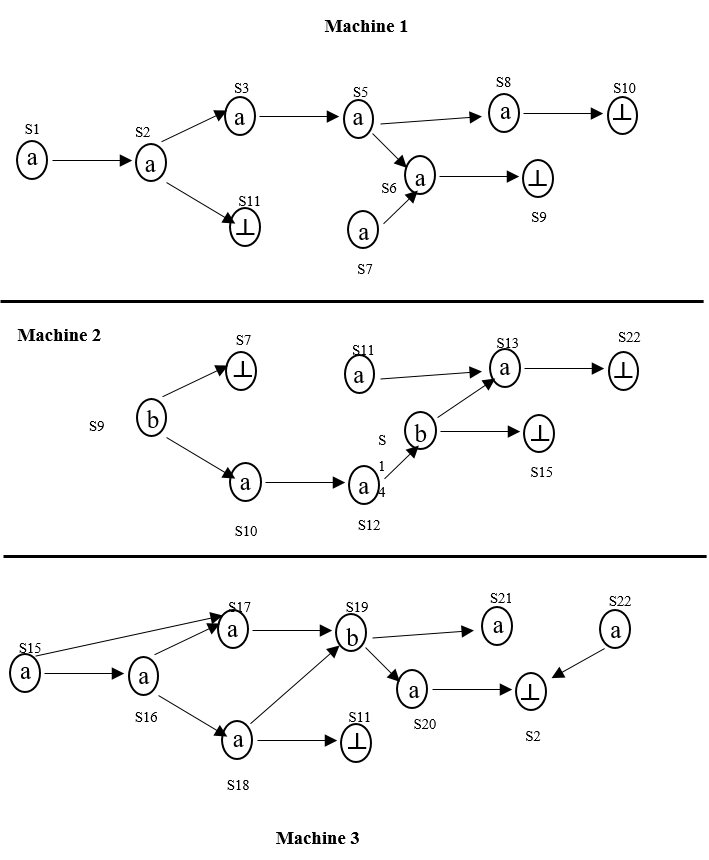
\includegraphics[height=4in]{img/skd2.png}	
	\captionof{figure}{Structure de kripke distribu\'{e}} \label{skd2}
	\end{center}

